\documentclass[12pt]{article}
\usepackage[utf8]{inputenc}
\usepackage{graphics}
\usepackage{graphicx}
\usepackage{float}
\usepackage{eso-pic}
\usepackage[top=3cm,bottom=3cm,left=2.5cm,right=2.5cm,headsep=10pt,letterpaper]{geometry}
\usepackage{verbatim}
\usepackage{amssymb}
\usepackage{stmaryrd}
\usepackage{mathrsfs, amsmath}
\usepackage{listings}
\usepackage{indentfirst}
\usepackage{tabularx}
\usepackage{hyperref}
\lstset{language = MATLAB}
\usepackage{abstract}
\usepackage{amsmath}
\usepackage{amsthm}
\usepackage{tcolorbox}
\usepackage{enumitem}

\begin{document}

\newpage
\newpage
\newtheorem{theorem}{Theorem}

\begin{titlepage}

    \begin{center}
        \vspace*{2.5in}
            \huge
            \textbf{{Homework 2}}\\
            \large
            \textbf{Numerical PDEs}\\
    \end{center}
    ~\vfill
    \noindent \textsc{Colorado School of Mines}\\
    \textsc{Department of Applied Mathematics and Statistics}\\
    
    \vspace{1cm}
    \noindent \textsc{\textbf{AUTHOR INFORMATION}}\\
    \noindent Hugh Scribner\footnote{Computational and Applied Mathematics}\\ 
    \vspace{1mm}
    
\end{titlepage}

\newpage

\tableofcontents

\newpage

\newpage
\section{Problem 1}
 \begin{tcolorbox}
        \textbf{Problem Statement:}\\
        Write finite difference solver to find the solution to the below PDE:
        \begin{align*}
            \text{\underline{PDE}}: \nabla^2u &= -8\cos(2x)\sin(2y),\\
            \text{\underline{BCs}}: u(0,y) &= u(\pi,y) = \sin(2y),\\
            u(x,0) &= u(x,\pi) = 0.
        \end{align*}
    \end{tcolorbox}
    
    \textbf{Solution:}\\
    My code from homework 0 does not generalize well to solving other problems, so I wrote a new one that defines A as a linear operator and solves the system using GMRES. Below are the results of some numerical experiments that confirm the new script reproduces the results of the old one.

        \begin{figure}[H]
        \begin{centering}
            \centering
                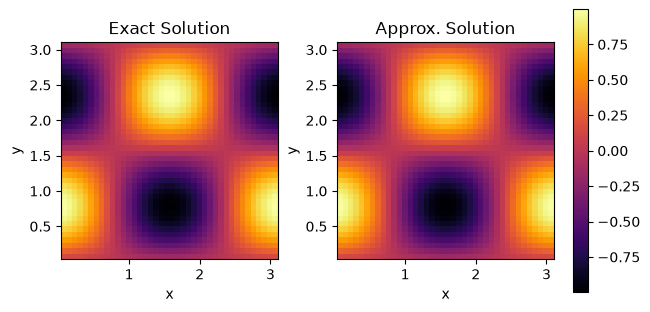
\includegraphics[scale=.75]{Images/problem_1/problem4_1.png}
                \caption{The figure above depicts the error in the FD approximation to the solution of the Poisson Equation.}
        \end{centering}
        \end{figure}

        \begin{figure}[H]
        \begin{centering}
            \centering
                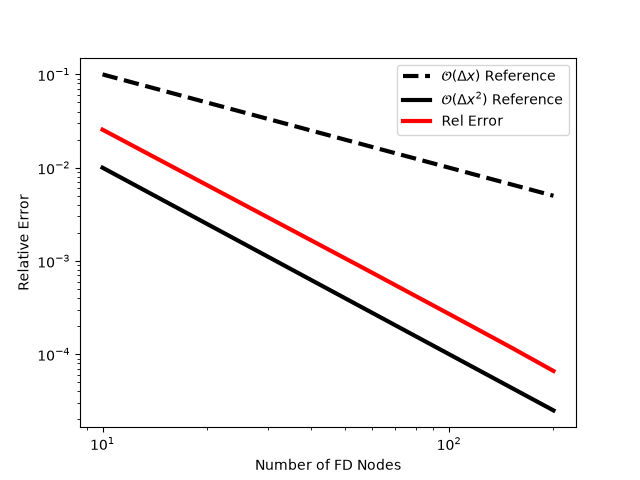
\includegraphics[scale=.75]{Images/problem_1/convergence_plot_4_1.png}
                \caption{The new script still attains $\mathcal{O}(dx^2)$ error with respect to the step size of the mesh.}
        \end{centering}
        \end{figure}

    
\newpage
\section{Problem 2}
 \begin{tcolorbox}
        \textbf{Problem Statement:}\\
        Using the Immersed boundary method, solve the same PDE as Problem 1, but add a circular boundary in the center such that $u(x,y) = cos(2x^{ib})sin(2y^{ib})$. Do some error testing to show the new model converges to the correct solution.

    \end{tcolorbox}
    
    \textbf{Solution:}\\

    Under the new boundary conditions, figure 3 shows that the numerical solution converges to what appears to be the correct solution.

    \begin{figure}[H]
        \begin{centering}
            \centering
                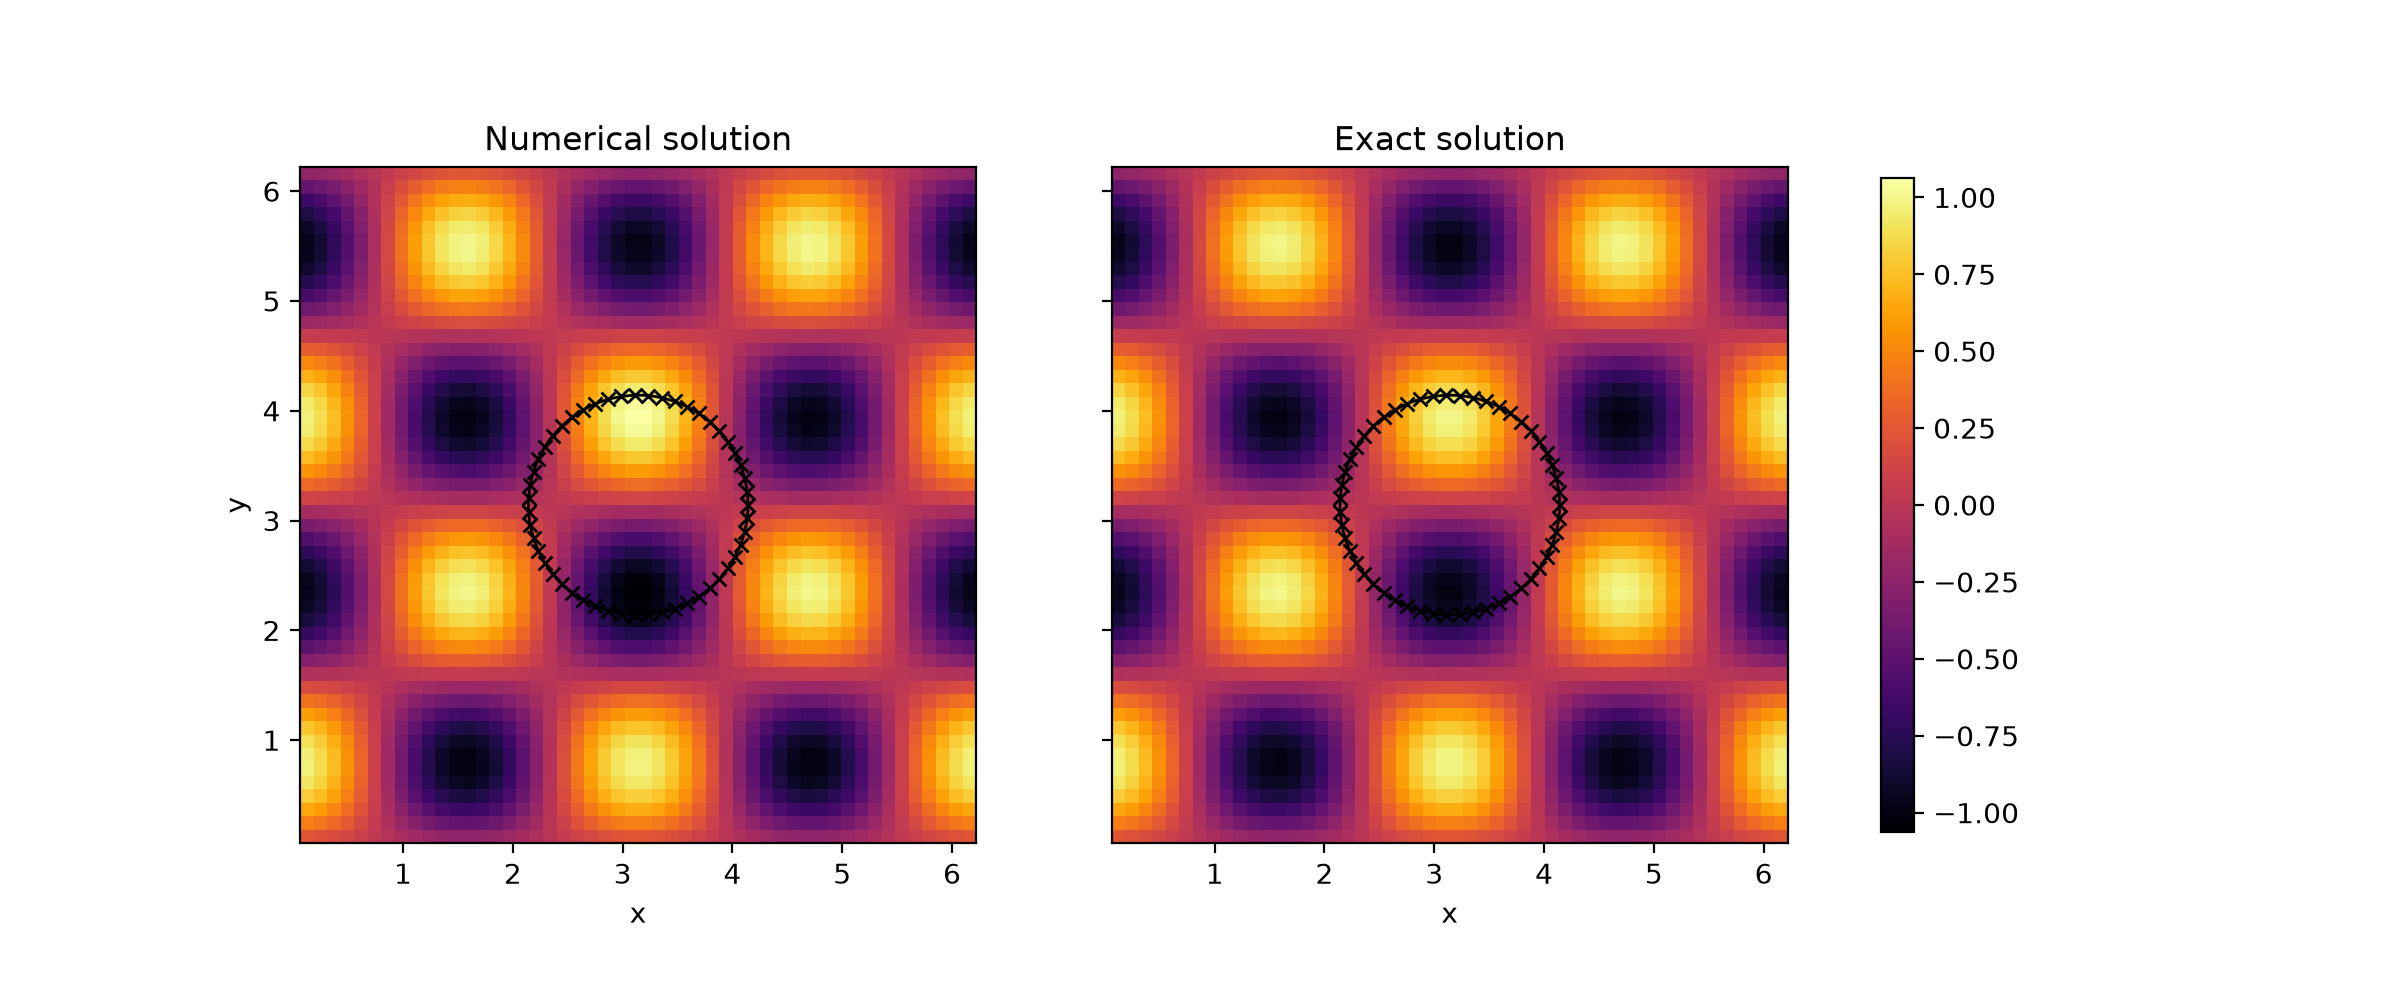
\includegraphics[scale=.5]{Images/problem_2/solution_comparison.png}
                \caption{From the perspective of the eyeball norm, the immersed boundary solution appears to approach the expected solution.}
        \end{centering}
    \end{figure}

    Looking a bit closer, we can inspect the absolute error between the exact and numerical solutions. For a mesh with N = 2500, the largest maximum error is .08.

    \begin{figure}[H]
        \begin{centering}
            \centering
                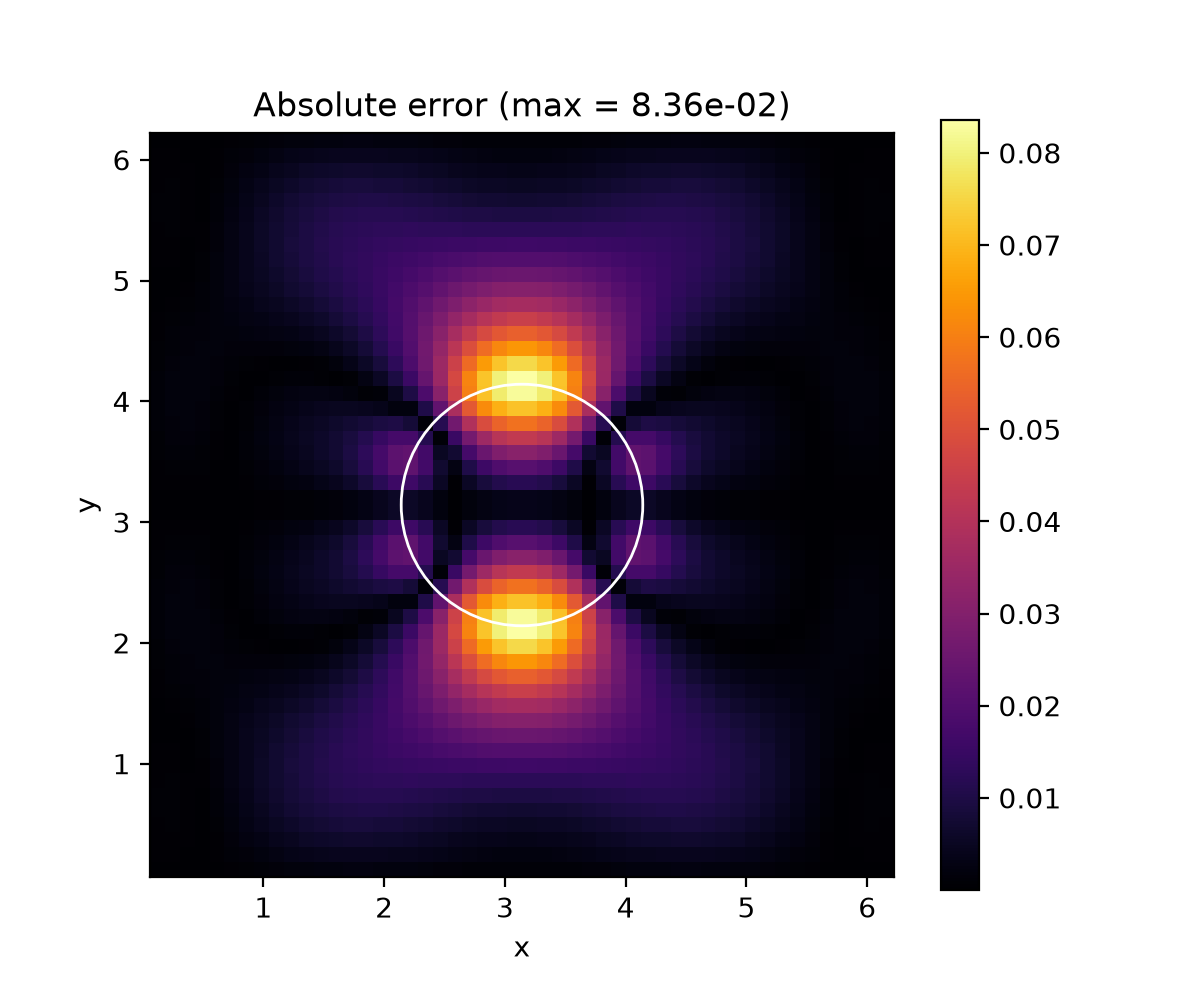
\includegraphics[scale=.5]{Images/problem_2/error.png}
                \caption{An absolute error plot shows a maximum error of .08 with a mesh of N=2500.}
        \end{centering}
    \end{figure}

    Evaluating the asymptotic behavior of the model, we find that the immersed boundary solver achieves a convergence rate of $\mathcal{O}(dx^2)$. This is unexpected, as the immersed boundary method typically demonstrates a convergence rate of $\mathcal{O}(dx^{1.5}$. We observe a superior convergence rate here due to the choice of test problem - since the boundary conditions along the immersed boundary match the exact solution to the corresponding Laplace equation exactly, the boundary weights all go to zero. This drives the system from the immersed boundary formulation to the more strongly convergent laplace solver.

    \begin{figure}[H]
        \begin{centering}
            \centering
                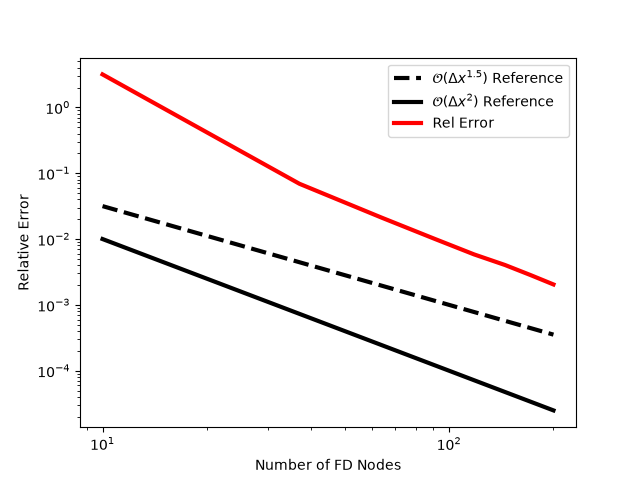
\includegraphics[scale=.75]{Images/problem_2/convergence_plot_4_2.png}
                \caption{The immersed boundary solver acheives non-characteristic $\mathcal{O}(dx^2)$ convergence.}
        \end{centering}
    \end{figure}

\newpage
\section{Problem 3}
 \begin{tcolorbox}
        \textbf{Problem Statement:}\\
        Now set all of the outer boundary conditions to zero and remove the forcing term from the PDE. What does the solution look like?
    \end{tcolorbox}
    
    \textbf{Solution:}\\
        Adjusting the boundary conditions to solve the near-minimal surface problem, the following surface solves the problem, isn't it pretty?

        \begin{figure}[H]
            \begin{centering}
                \centering
                    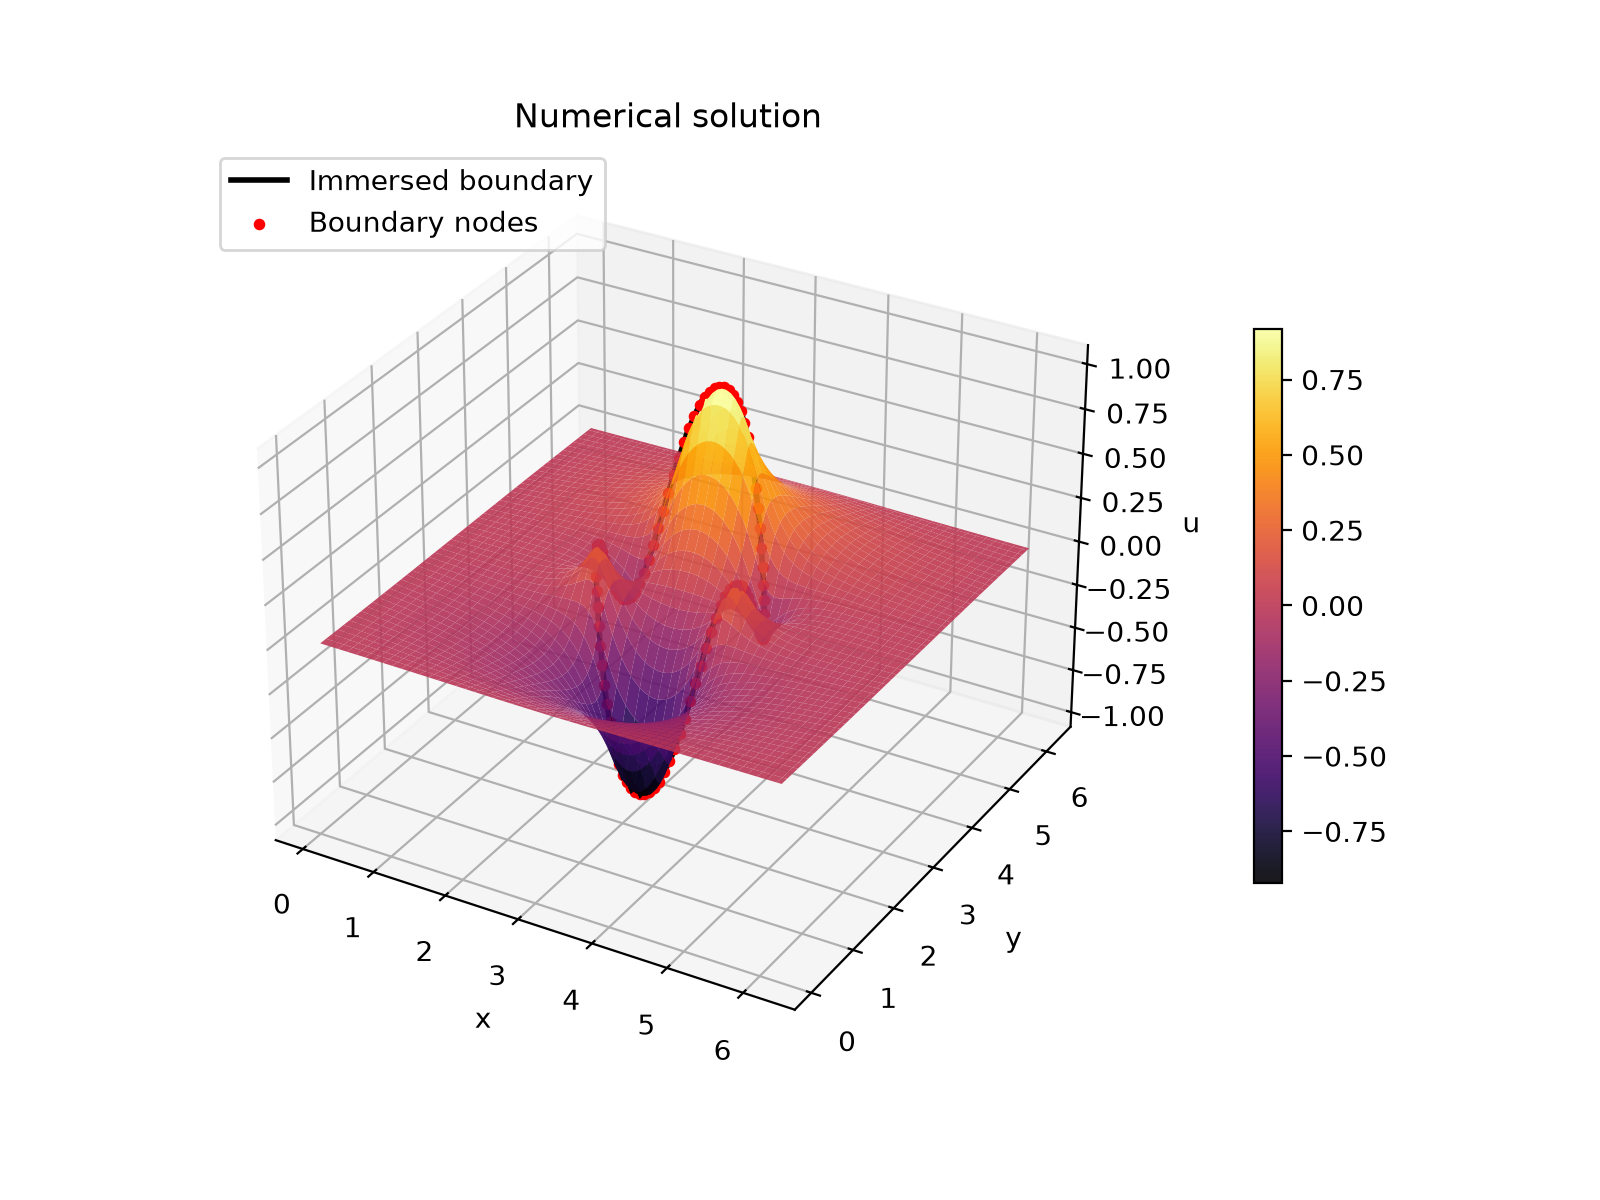
\includegraphics[scale=.75]{Images/problem_3/surface.png}
                    \caption{Numerical solution to the near minimal surface problem on a mesh with N = 10000.}
            \end{centering}
        \end{figure}

    We can play with the number of nodes used to represent the immersed boundary. Notably, assembling each nodes contribution to the corresponding linear system is by far the most expensive part of solving this problem aside from the linear solve, so adding a large number of nodes severly impacts the run time of the simulation. Likewise, if we use too few nodes, we may find that the boundary is not accurately enforced on the problem. To test this I ran the code with 1/10th of the nodes as the previous simulation As you can see, the peak of the minimal surface is now bifurcated, so we had too few nodes to get a sensible solution.

        \begin{figure}[H]
            \begin{centering}
                \centering
                    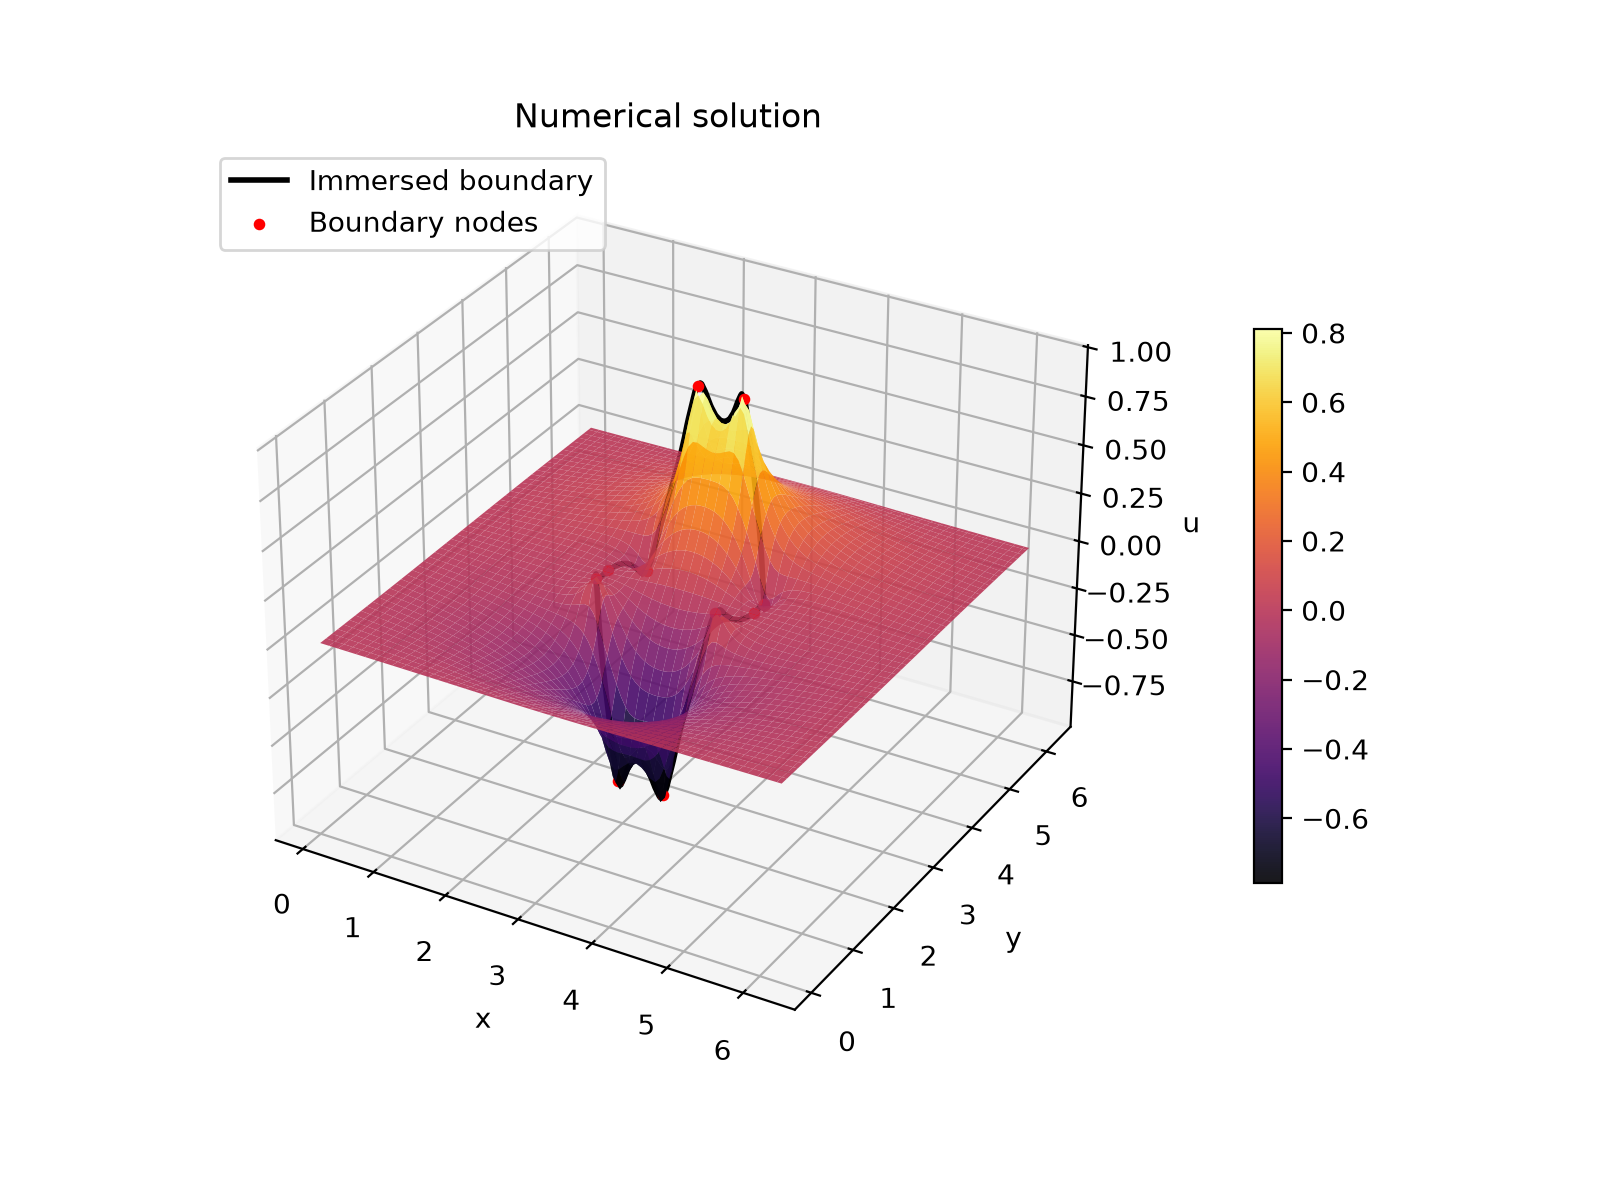
\includegraphics[scale=.75]{Images/problem_3/surface_few_grid points.png}
                    \caption{If we choose to use a small number of boundary nodes, non-physical peaks begin to appear in the numerical approximation.}  
            \end{centering}
        \end{figure}

\newpage
\section{Problem 4}
 \begin{tcolorbox}
        \textbf{Problem Statement:}\\
        Do something fun with your code!
    \end{tcolorbox}
    
    \textbf{Solution:}\\
        We can introduce some pseudo dynamics to this problem by updating the boundary conditions of the mesh such that $u(x^{ib}(t), y^{ib}(t)) = f(t)$ and then applying the laplace solver over a discretized series of time steps. While this may yield some non-physical dynamics for our system (I'm almost certain any real problem where the non-minimal surface equation would pop up will begin its derivation with "assume stationary point charges"), it will definitely yield some pretty visually interesting videos. 

        In my exploration I tried two new sets of boundary condtions; A rotating circle around the origin and an expanding and contracting circle about the origin.
        \begin{subequations}
            \begin{align}
                u(x^{ib}(t),y^{ib}(t)) &= \cos(2x^{ib}(t))\sin(2y^{ib}(t))\\
                x^{ib} &= \cos(\theta) + \cos(2\pi t)\\
                y^{ib} &= \sin(\theta) + \sin(2\pi t) \quad \theta = [0, 6\pi] \quad t = [0, 6]\\
            \end{align}
        \end{subequations}
        and 
        \begin{subequations}
            \begin{align}
                u(x^{ib}(t),y^{ib}(t)) &= \cos(2x^{ib}(t))\sin(2y^{ib}(t))\\
                x^{ib} &= (1+.5\cos(2\pi t))\cos(\theta) + \\
                y^{ib} &= (1+.5\cos(2\pi t))\sin(\theta) \quad \theta = [0, 6\pi] \quad t = [0, 6]\\
            \end{align}
        \end{subequations}
        If you would like to see the videos generated by the code, they can be found in the movies folder of the associated \href{https://github.com/Hugh-Scribner/Math550_HW2/tree/main/Movies}{github repo}. The results from (1) are associated with the "moving\_center\_movie.mp4", while the results from (2) are in "moving\_radius\_movie.mp4". Enjoy!
\end{document}
